\chapter{Introducción: Optimización de los datos de un EEG}\label{cap:QEEG}

\section{Panorama actual}

La optimización de los datos de un electroencefalograma, a partir de ahora EEG por sus siglas en inglés, está dentro de la categoría de problemas de Big Data, problemas donde no sólo el tamaño del mismo supone de por si una dificultad, sino que también influyen aspectos como el ruido en los datos, la no existencia de patrones fácilmente reconocibles o restricciones de tiempo inherentes al problema.

En el año 2015 se presenta este problema como candidato a conformar la base del \textbf{Optimization of Big Data Competition - CEC 2015}\cite{EvolutionaryBigOpt}, donde se realiza su estudio a través de dos algoritmos multiobjetivo muy potentes, cuyos resultados, a pesar de catalogarse como satisfactorios, demostraron que era necesario disponer de mejores propuestas y métodos que aportasen un rendimiento superior en términos de tiempo y calidad de las soluciones.

Para entender mejor los orígenes del problema hace falta hacer un breve repaso por la utilidad real que tienen los EEGs en distintas áreas de conocimiento, principalmente para comprender porqué es tan importante disponer de técnicas de resolución eficientes. En ámbitos médicos como la neurociencia se utilizan dispositivos denominados BCI (Brain-computer Interfaces)\cite{BCI} que se encargan de \textbf{capturar la actividad cerebral} a través de electrodos, con el fin de analizar estos datos, procesarlos y traducirlos en acciones o estados cognitivos que puedan utilizarse para actuar en consecuencia ante una determinada situación, como puede ser para diagnosticar distintas enfermedades del sistema nervioso central.

Los BCIs hacen uso principalmente de los \textbf{electroencefalogramas} (EEG), que son exploraciones neurofisiológicas que registran la actividad bioeléctrica cerebral, concretamente de las neuronas, a través de electrodos (componentes de los BCIs), con el objetivo principal de detectar y diagnosticar enfermedades o trastornos del sistema nervioso central\cite{EEG}, tales como epilepsia, daños cerebrales de distintos tipos, trastornos psiquiátricos, encefalopatías y demás afecciones\cite{EEG2}, así como para potenciar las capacidades cognitivas frente a determinadas situaciones\cite{ICA-EGG}.

Ciertos campos de estudio y aplicaciones en concreto utilizan lo que se conoce como \textbf{electroencefalografía cuantitativa}, QEEG \cite{QEEG}, que por medio de una malla de electrodos registra de \textbf{forma simultánea} los impulsos eléctricos de \textbf{múltiples partes del cerebro}. Decodificar de forma efectiva y eficiente estos QEEG en \textbf{estados cognitivos de orden superior}\cite{EvolutionaryBigOpt}, como pueden ser emociones, recuerdos o estados cerebrales, promovería la creación de BCIs más avanzados que sustenten el uso de estos sistemas tanto en el tratamiento de pacientes con distintos trastornos del sistema nervioso como para las actividades del día a día, sobre todo de aquellas que conlleven la toma de decisiones críticas en tiempo real, como por ejemplo, el control del tráfico aéreo \cite{EEG-AirTraffic}.

Sin embargo, el correcto funcionamiento de los BCIs se ve normalmente truncado por dos principales aspectos: la cantidad de \textbf{información cerebral \textit{real}} que es captada y la \textbf{distorsión que producen las señales eléctricas no cerebrales}, lo que se denominan \textbf{artifacts}, y que quedan plasmadas en el EEG cuantitativo, empañando los resultados obtenidos y elevando la complejidad del proceso de decodificación. Es aquí donde entran en juego técnicas como el \textbf{Análisis de Componentes Independientes, ICA}, y otras técnicas que se encargan de separar la señales obtenidas de distintas fuentes. 

Finalmente, tras un proceso de inspección visual llevado a cabo actualmente por un ser humano, se eliminan los artifacts de las componentes resultantes y se recompone el EEG original. Naturalmente, esta tarea se vuelve \textbf{totalmente inviable} de cara a los procesos de obtención de QEEG actuales, donde se requiere inspeccionar grandes cantidades de datos, lo que consume mucho tiempo y reduce la eficiencia del proceso. Es por esta principal razón por la que se requieren de técnicas eficaces que permitan \textbf{automatizar el proceso} y \textbf{reducir la intervención humana}, en aras de una optimización mucho mas eficiente. La figura \ref{fig:EEGData} muestra un ejemplo de EEG, en una propuesta que contempla la eliminación de artifacts oculares a través del procedimiento ICA.

\begin{figure}[h]
	\centering
	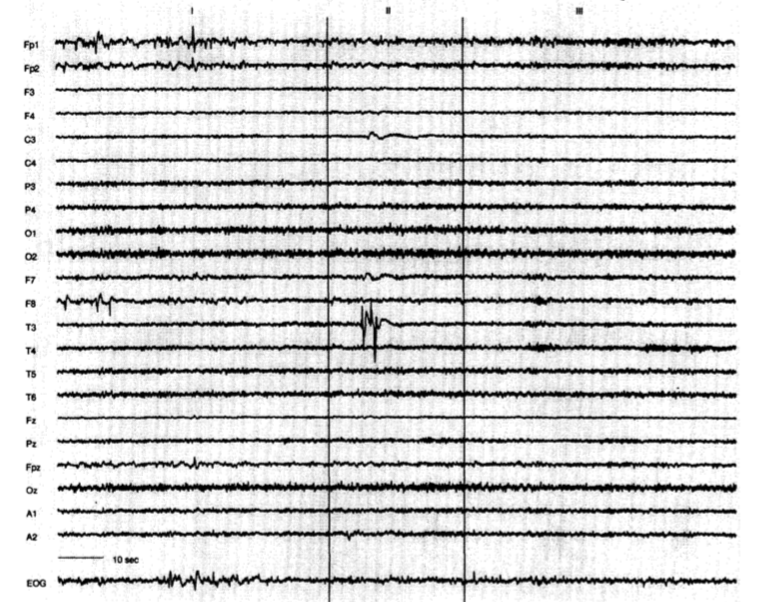
\includegraphics[scale=0.45]{imagenes/EEGData}
	\caption{EEG: Estudio de eliminación de artifacts oculares a través de ICA. Fuente \cite{EEG-Eye}} 
	\label{fig:EEGData}
\end{figure}

La propuesta recogida en \cite{EvolutionaryBigOpt} provee una forma de representar el problema de la decodificación de un QEEG, de forma que cualquier técnica, método o algoritmo preparado para el procesamiento de grandes cantidades de datos y la optimización global de miles de variables, pueda ser sometido a pruebas exhaustivas frente a este problema real, y finalmente sugerir, si cabe, un posible candidato que sustituya al actual método de decodificación, descrito en el párrafo anterior, con el último fin de dar un salto importante en el diseño de sistemas BCIs para la mejora de la calidad de vida de todas aquellas personas que lo requieran.

Como el estudio se basa completamente en la clara definición del problema en cuestión, los siguientes párrafos contendrán toda la información referente a éste, desde la representación elegida, pasando por las bases de datos disponibles y llegando hasta la definición de la función objetivo que marcará el camino a seguir en este estudio. Como aclaración, se habla de QEEG como un tipo de EEG utilizado en algunos campos, aunque a efectos prácticos para entender y describir el problema, se les considera equivalentes.

\section{Representación del problema: EEG}

Para definir el problema de la optimización de un EEG se ha empleado una representación que divide al problema en 3 subproblemas con la misma naturaleza que el original, donde únicamente cambian la dimensión del mismo y la existencia de ruido en los datos. De esta forma, se ha generado una base de datos sintéticos (generados de forma artificial)\cite{ICA-Calibrate} que se reúnen en tres Datasets \textbf{A, B y C} tal y como se muestra en la siguiente tabla.

\begin{table}[H]
	\centering
	\resizebox{\textwidth}{!}{
		$\begin{tabular}{ *{5}{c}}
		\toprule
			\textbf{Dataset}& \textbf{Nº Fuentes} & \textbf{Nº Artifacts} & \textbf{Sin ruido} & \textbf{Con ruido} \\
			\midrule
			\textbf{A} & 4 & 2 & D4 & D4N\\ 
			\textbf{B} & 12 & 6 & D12 & D12N \\ 
			\textbf{C} & 19 & 6 & D19 & D19N \\ 
			\bottomrule
		\end{tabular}$
	}
		\caption{Grupos del problema del EEG.}
		\label{tabla:gruposEEG}
\end{table}

Cada dataset propone una dificultad distinta en términos del número de fuentes de señales reales y de ruido con una \textbf{varianza de 0.1}. Las fuentes de señales efectivas son la suma del \textbf{número de fuentes de datos reales} y el \textbf{número de artifacts}, donde estos últimos operan en altas frecuencias y amplitudes. 

Las señales de los artifacts \textbf{simulan impulsos electromagnéticos} que se generan de forma involuntaria con movimientos de cualquier parte de nuestro cuerpo durante el tiempo en el que se recogen los datos en el EEG, y al ser señales eléctricas, son captadas por éste mezclándose con las señales reales de nuestro cerebro y empañando el EGG. Cada señal se muestrea a una frecuencia de \textbf{256Hz,} y los artifacts son activados en intervalos que oscilan entre los últimos \textbf{250ms-500ms} de cada segundo (ver \cite{ICA-Calibrate}).

Para el \textbf{Dataset A}, las 6 señales totales se mezclan en \textbf{4 señales de datos}, $\vv{x_1}, \vv{x_2}, \vv{x_3}$ y $ \vv{x_4} $ compuestas según las siguientes ecuaciones, donde las señales 5 y 6 son artifacts.

\begin{equation}\label{eq:D4}
	\begin{gathered}
		\vv{x_1} = \vv{s_1} + 0.9\vv{s_5}\\
		\vv{x_2} = \vv{s_2} + 0.9\vv{s_6}\\
		\vv{x_3} = \vv{s_3} + \vv{s_5}\\
		\vv{x_4} = \vv{s_4} + \vv{s_6}\\
	\end{gathered}
\end{equation}

Para los \textbf{Datasets B y C}, las 6 señales de artifacts se disparan en posiciones determinadas de la cabeza de una persona, indicadas  en la figura \ref{fig:artifactsLocation}. De forma análoga, cada fuente de datos real de las 12 (Dataset B) o 19 (Dataset C) se mezcla con cada una de las $k$ fuentes de artifacts siguiendo la ecuación:

\begin{equation}\label{eq:D12-9}
	\begin{gathered}
	\vv{x_i} = \vv{s_i} + \sum_{k=1}^{N} w_{ik} s_k\\
	w_{ik} = exp (-r^2)
	\end{gathered}
\end{equation}

donde $w_{ik}$ representa el exponencial de la distancia Euclídea al cuadrado con signo negativo de la señal \textit{i-ésima} y el artifact \textit{k-ésimo}. Esta distancia se calcula teniendo en cuenta la posición donde se colocan los electrodos (fuentes de datos reales) y desde donde se disparan los artifacts en una cabeza de radio 0,5dm, tal y como se puede ver en la figura.

\begin{figure}[h]
	\centering
	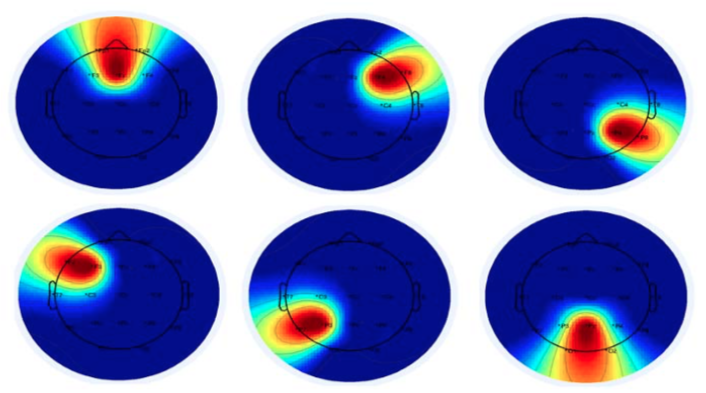
\includegraphics[scale=0.45]{imagenes/Artifacts}
	\caption{Disposición de los 6 artifacts y la contribución de cada uno en todos los electrodos. Fuente: \cite{EvolutionaryBigOpt}}
	\label{fig:artifactsLocation}
\end{figure}

En resumen, un total de \textbf{6 problemas distintos}, \textbf{D4, D4N, D12, D12N, D19 y D19N}, donde cada señal se muestrea a 256Hz, da lugar a \textbf{tres valores de dimensionalidad del problema} que repercuten directamente en la complejidad en cuanto a espacio de soluciones, donde cada dimensión se calcula como el \textbf{número de señales de entrada ($N$)} de cada problema multiplicada por la \textbf{frecuencia de muestreo (256Hz)}. Con esta definición se busca facilitar la representación interna de las soluciones como un único conjunto de variables a optimizar; así, el \textbf{Dataset A} tiene \textbf{1024} variables, el \textbf{Dataset B} cuenta con \textbf{3072} y el \textbf{Dataset C} concretamente dispone de \textbf{4864} variables.

Esta elección conceptual conforma la base de este estudio a nivel de representación de los datos, lo que permitirá evaluar el grado de desempeño de un algoritmo frente a la optimización de los datos simulados de un EEG, cuyos resultados son extrapolables a una aplicación médica real si se tiene en cuenta el proceso matemático y estadístico sobre el que se sustenta la decodificación de las señales medidas y que se describe a continuación.

\section{ICA: Independent Component Analysis}

Un Análisis de Componentes Independientes, \textbf{ICA} en inglés, es un método de procesamiento de señales utilizado principalmente para eliminar artifacts \cite{ICA-Calibrate}. Permite \textbf{separar en fuentes de datos independientes} aquellas fuentes que han sufrido transformaciones lineales y se encuentran mezcladas, a través de una maximización de la independencia estadística de las componentes resultantes\cite{ICA-EGG}.

A grandes rasgos un ICA consta de dos pasos, un primer paso donde se elimina toda la correlación de los datos, llamado \textit{data whitening}, y un segundo paso donde se aplica la matriz de rotación inversa a la transformación aplicada, con el fin de obtener los datos originales. La correlación de los datos se debe principalmente a que un electrodo localizado en una parte determinada de la cabeza, no sólo medirá los impulsos eléctricos de esa zona en particular, sino que también se verá afectado por las señales cercanas que estén siendo sensadas por otros electrodos. 

 Expresado de forma matemática, un ICA busca una \textbf{transformación lineal V} de los \textbf{datos D} de forma tal que $P = V\cdot D$ y que $Cov(P) = I$, siendo $Cov$ la matriz de covarianza e $I$ la matriz de identidad, lo que indica que las variables no tienen correlación alguna (paso 1, \textbf{data whitening}). Tras encontrar $V$, se procede a realizar la rotación de la matriz a través de la \textbf{minimización de la Gaussianidad} de la matriz en cuestión.
 
 Por tanto, el problema de la optimización del EEG se puede formular análogamente a la aplicación de un ICA de la siguiente manera:
 
 \begin{equation} \label{eq:problem1}
	 \begin{gathered}
		X = A\cdot S + N
	 \end{gathered}
 \end{equation}
 
 donde $X$ es la matriz combinada de señales (debido a la naturaleza de la medición), A es la matriz de combinación que representa la transformación lineal \textit{V} del ICA al combinarse las señales entre sí, \textit{N} es el ruido y \textit{S} las fuentes de datos originales; así al disponer de \textit{A} y unas fuentes estimadas $\hat{S}$, hay que encontrar \textit{W} tal que $\hat{S} = W\cdot X$. Finalmente se reconstruyen las señales limpias a través de las componentes útiles, tal que : $\hat{X} = W^{-1} \hat{S}$
 
 \section{Formulación del problema: enfoque uniobjetivo}
 
 La formulación original del problema sigue un enfoque multiobjetivo pero adoptar un \textbf{enfoque uniobjetivo} reduce la complejidad del problema sin incurrir en pérdida alguna de generalidad. Por tanto, se utilizará el enfoque multiobjetivo para formular el problema pero experimentalmente se generalizará a uno uniobjetivo.
 
 Sea \textit{X} (matriz combinada de señales) una matriz de dimensión $n\times m$ donde $n$ es el número de \textbf{series de tiempo interdependientes} y $m$ la \textbf{longitud} de cada serie. Sea a su vez \textit{S} (matriz de fuentes reales) una matriz $n\times m$ con $n$ series de tiempo \textbf{independientes} de longitud $m$ y \textit{A} una \textbf{matriz de transformación lineal} $n\times n$. Se sabe que:
 
  \begin{equation}
	 \begin{gathered}
	 	X = A\times S
	 \end{gathered}
 \end{equation}
 
 Por tanto el problema consiste en descomponer S en $S_1$ y $S_2$ tal que $S = S_1 +S_2$ y que además $X = A\times S_1 + A\times S_2$. Y sea $C$ la matriz de \textbf{coeficientes de correlación de Pearson} entre $X$ y $A\times S_1$ definida como:
 
 \begin{equation} \label{eq:covar}
	 \begin{gathered}
	 	C = \frac{covar(X,AS_1)}{\sigma(X)\cdot \sigma (A\cdot S_1)}
	 \end{gathered}
 \end{equation}
 
 donde $covar( )$ representa la matriz de covarianzas y $\sigma$ la varianza.
 El objetivo consiste en \textbf{maximizar los elementos diagonales de C} a la vez que se minimizan los elementos de fuera de la diagonal, y conseguir que la \textbf{distancia entre $S$ y $S_1$} sea la mínima posible, lo que a su vez maximice la similitud entre estas \cite{EvolutionaryBigOpt}. Para ello, se debe encontrar una matriz $S_1$ que minimice el valor de las siguientes funciones:
 
  \begin{equation} \label{eq:function1}
	 \begin{gathered}
	 	Minimize \ f_1 = \frac{1}{N^2 -N} \sum_{i}^{} \sum_{j \neq i}^{} C_{ij}^2 + \frac{1}{N} \sum_{i}^{} (1-C_{ii})^2
	 \end{gathered}
 \end{equation}
 
  \begin{equation} \label{eq:function2}
	 \begin{gathered}
	 	Minimize \ f_2 = \frac{1}{N \times M} \sum_{i}^{} \sum_{j}^{} (S_{ij} - S_{1ij})^2
	 \end{gathered}
 \end{equation}
 
 donde se busca \textbf{eliminar la mayor cantidad de artifacts posibles} a la vez que se \textbf{minimiza la pérdida de información real}. A través de estas dos funciones se propone el  \textbf{enfoque uniobjetivo} donde la función objetivo a optimizar es la siguiente:
 
 \begin{equation} \label{eq:FObj}
	 \begin{gathered}
	 	f = Minimize(f_1 + f_2)
	 \end{gathered}
 \end{equation}
 
 Queda definida por tanto la base sobre la que se construye este estudio, donde la función objetivo juega un papel principal en cuanto al problema de la optimización de los datos de un EEG. En el siguiente capítulo será revisada la literatura del problema en cuestión, además del conjunto de problemas más utilizados actualmente para la evaluación de los algoritmos, los denominados benchmarks, y por último los principales algoritmos y técnicas utilizados para problemas de tipo \textbf{LSGO}.